\chapter{Aufgabe 1 }
\section*{a}
Die Methode gibt die Anzahl negativer Elemente plus der Elemente die mit v übereinstimmen, falls diese nicht negativ sind zurück. Falls ein Element von a[] am 2.,3.,oder 4. Bit eine 1 hat wird eine IllegalArgumentException geworfen.

\section*{b}
Siehe Abbildung \ref{fig:flowChart}.
\begin{figure}[h]
	\centering
	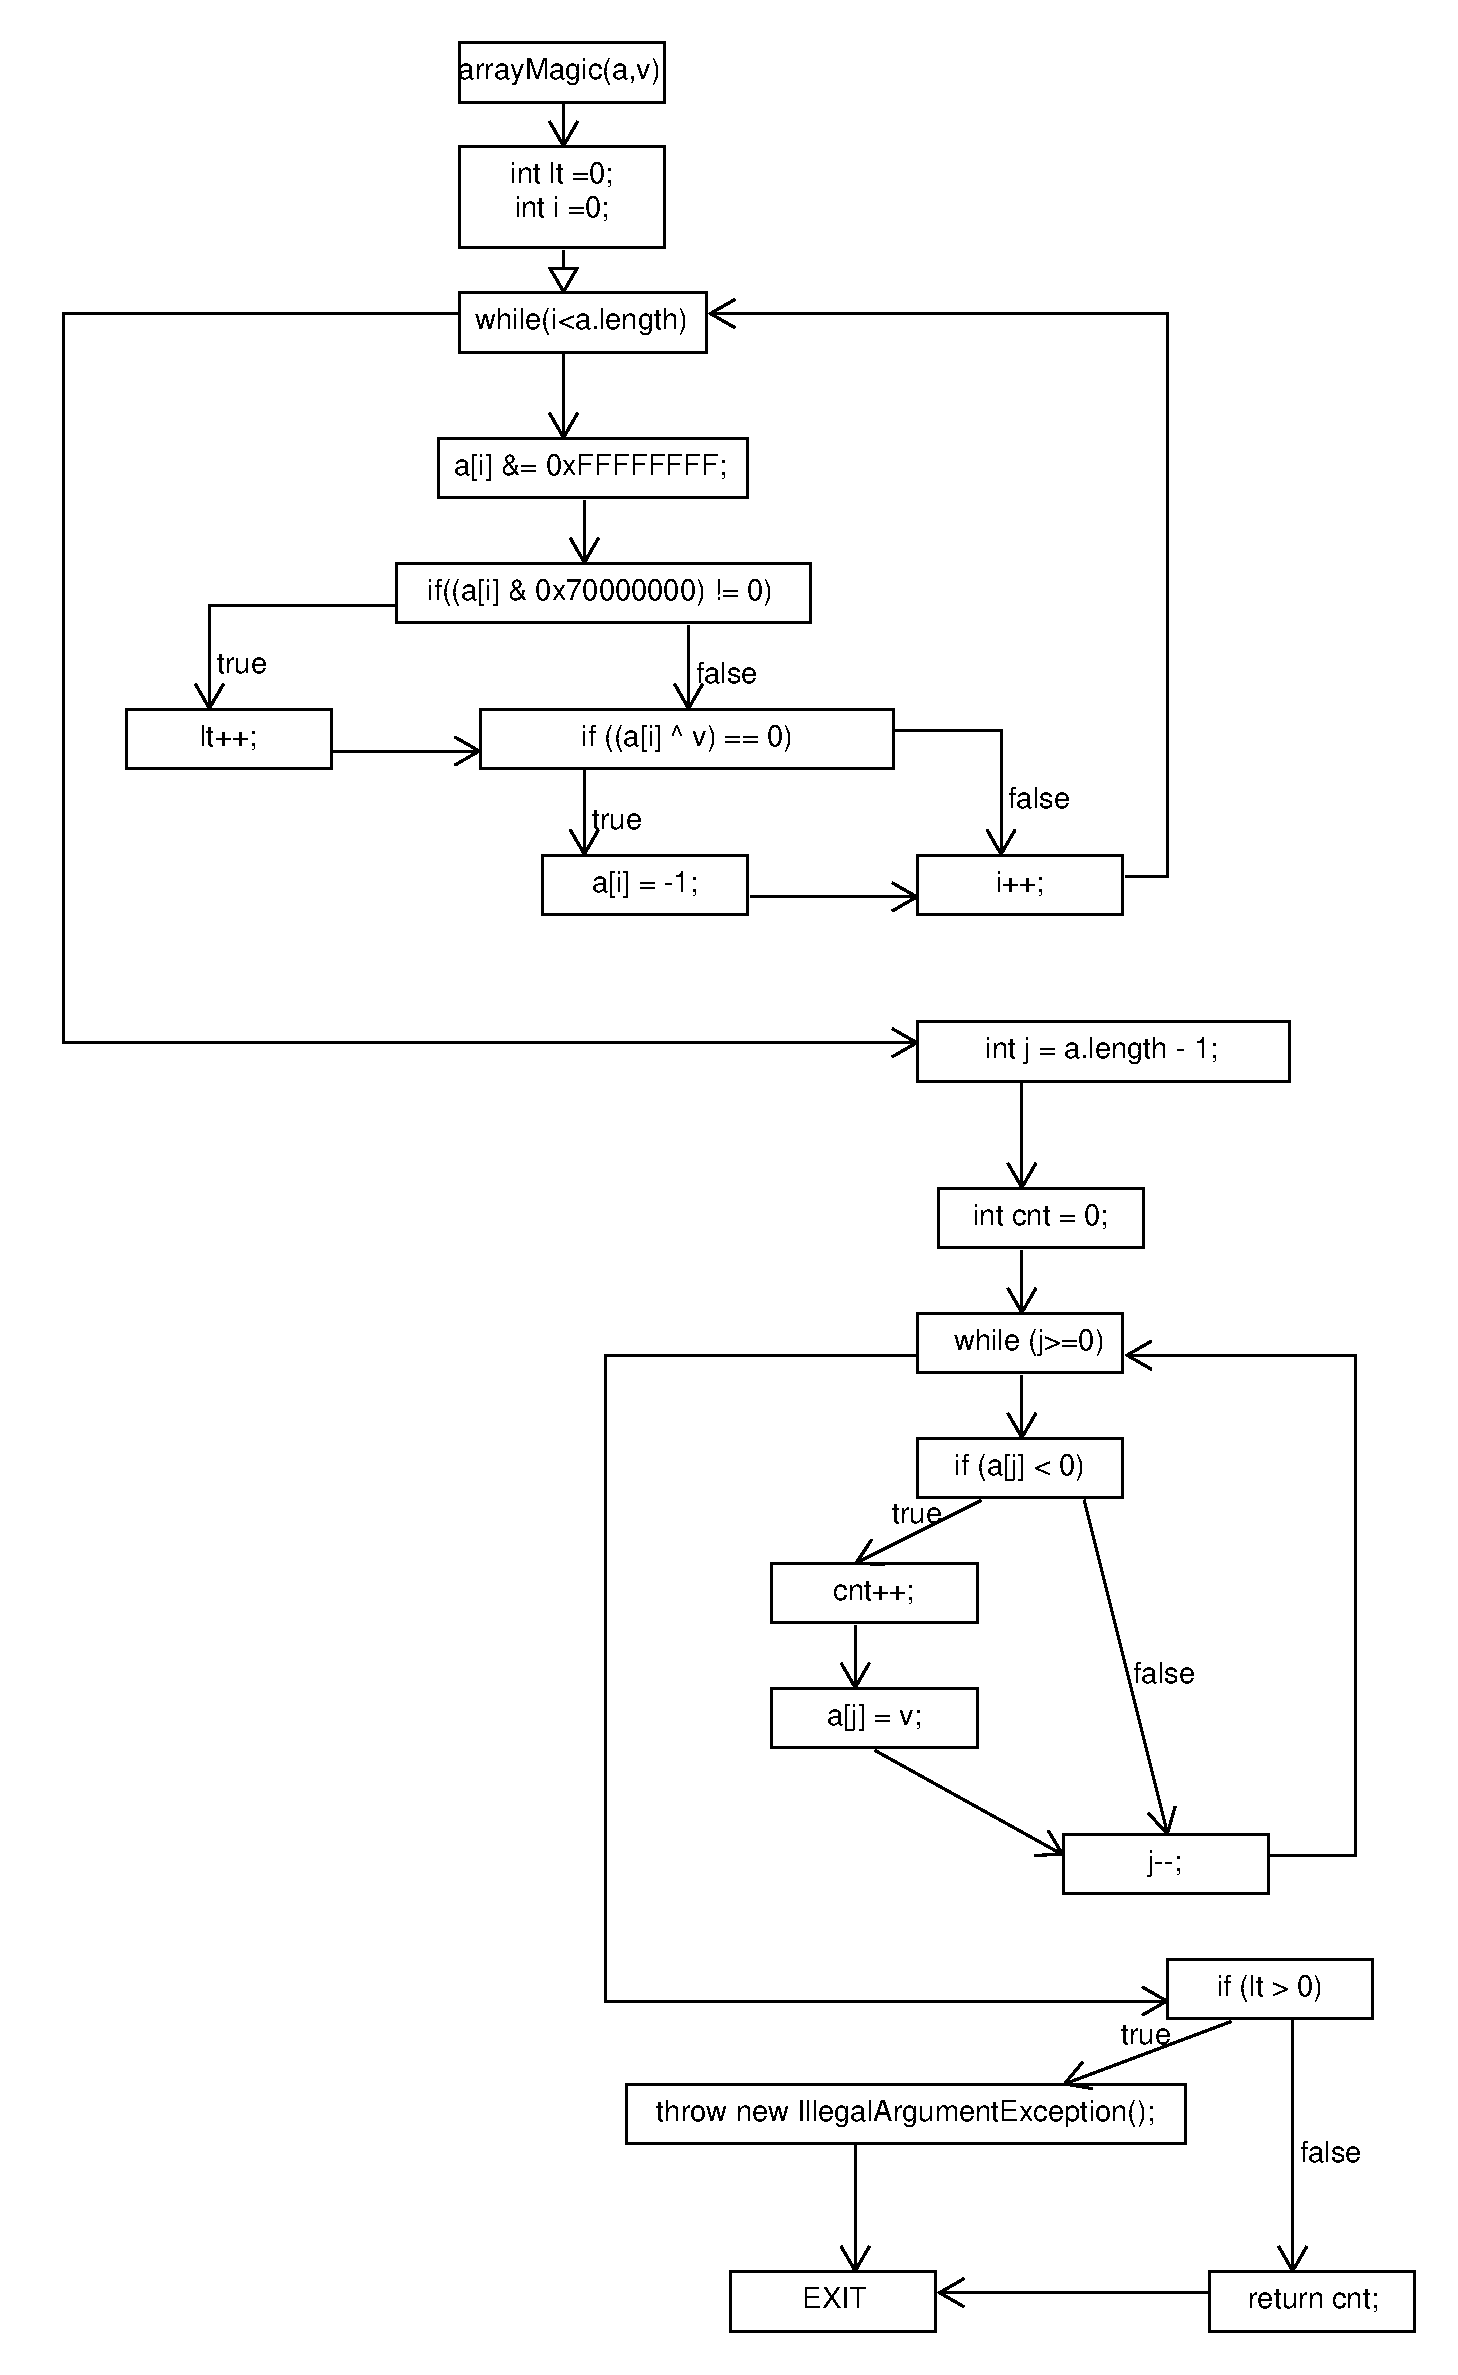
\includegraphics[width=0.8\textwidth, clip]{FlowChart.pdf}
	\caption{Kontrollflussgraph}
	\label{fig:flowChart}
\end{figure}
\section*{c}
Für die zyklomatische Komplexität nach der Formel $ C=E-N+2P$ ergibt sich mit den Werten
\begin{equation}
	C= 25-20+2 \cdot 1 = 7.
\end{equation}
Mit $C=7<10$ liegt die Komplexität zwar unter der kritischen Grenze, ist für einen Code mit einer so simplen Aufgabe jedoch sehr hoch. 
Da der Code zwei Mögliche Enden hat (eine Exception oder den Return) muss ein Exit Knoten eingeführt werden.



%Kanten:25
%Knoten:20
%P:2*1
%
%C = E-n+ 2P

\section*{d}
Die Zeile 7 erfüllt keinen Zweck. Denn werden alle 32 Bits eines Integers jeweils mit einer 1 Bitweise Und-Verknüpft, so erhält man wieder den selben Integer.
Die Zeile hat keinen Einfluss auf die Zyklische Komplexität, da Sie dem Graphen genau einen Knoten und eine Kante hinzufügt, was gemäß
\begin{align}
	C = (E + 1) - (N + 1) + 2P = E - N + 2P
\end{align}
zu keiner Änderung von $C$ führt.